\documentclass[10pt]{amsart}
\usepackage[paperheight=9.2in,paperwidth=6in,margin=0in]{geometry}
%\geometry{landscape}                % Activate for for rotated page geometry
%\usepackage[parfill]{parskip}    % Activate to begin paragraphs with an empty line rather than an indent
\usepackage{graphicx}
\usepackage{amssymb}
\usepackage{epstopdf}
\DeclareGraphicsRule{.tif}{png}{.png}{`convert #1 `dirname #1`/`basename #1 .tif`.png}

% LUKE'S SETTINGS
% packages
\usepackage{framed}
\usepackage{xcolor}
\usepackage{hanging}
% paragraph
\setlength\parindent{0pt}
\setlength{\parskip}{1em}
% margins
%\addtolength{\oddsidemargin}{0.25in}
\addtolength{\topmargin}{0.15in}
%\addtolength{\textheight}{3in}
% frame
\definecolor{shadecolor}{rgb}{0.95,0.95,0.95}
% fixed width font (Courier)
\renewcommand{\ttdefault}{pcr}
% san-serif font (Helvetica)
\usepackage[scaled]{helvet}
\renewcommand\familydefault{\sfdefault} 
\usepackage[T1]{fontenc}
% column widths with any alignment
\usepackage{array}
\newcolumntype{L}[1]{>{\raggedright\let\newline\\\arraybackslash\hspace{0pt}}m{#1}} % left-mid
\newcolumntype{C}[1]{>{\centering\let\newline\\\arraybackslash\hspace{0pt}}m{#1}}   % center-mid
\newcolumntype{R}[1]{>{\raggedleft\let\newline\\\arraybackslash\hspace{0pt}}m{#1}}  % right-mid
\newcolumntype{X}[1]{%
 >{\vbox to 2ex\bgroup\vfill}%
 p{#1}%
 <{\egroup}} 
 
% no extra space after period
\frenchspacing

% Macros file generated by trading_cards_2_macros_figures.ipynb
\def\sequence{TACGGAAGGTCCGGGCGTTATCCGGATTTATTGGGTTTAAAGGGAGCGTA
GGCCGTCTGTTAAGCGTGTTGTGAAATGTCGGGGCTCAACCTGGGCATTG
CAGCGCGAACTGGCAGACTTGAGTG}
\def\taxonomyGG{k\_\_Bacteria; p\_\_Bacteroidetes; c\_\_Bacteroidia; o\_\_Bacteroidales; f\_\_Prevotellaceae; g\_\_Prevotella; s\_\_stercorea}
\def\wikipedia{Prevotella is a genus of Gram-negative bacteria.
Prevotella spp. are members of the oral and vaginal flora, and are recovered from anaerobic infections of the respiratory tract. These infections include aspiration pneumonia, lung abscess, pulmonary empyema, and chronic otitis media and sinusitis.}
\def\prevalencePercent{1.34}
\def\prevalenceRank{971}
\def\abundancePercent{0.0223}
\def\abundanceRank{424}
\def\numOTUs{27248}
\def\trimLength{125}
\def\numSamples{9511}
\def\rarefactionDepth{1250}


% No page numbers
\thispagestyle{empty}

% Document
\begin{document}

%\begin{framed} % alt: shaded

%\vspace{-6mm}

\begin{center}

\includegraphics[width=12cm]{../agp_header.pdf}
\end{center}

\hspace{2cm}
\begin{tabular}{L{5in}}
\texttt{\sequence{}}
\end{tabular}

\begin{raggedright}
\begin{hangparas}{2em}{1}
    TAXONOMY: \taxonomyGG{}
    
    WIKIPEDIA:  \wikipedia{}

    PREVALENCE: Found in \prevalencePercent{}\% of 9,511 samples, %\numSamples{}
                rank \#\prevalenceRank{} out of 27,248 sequences. %\numOTUs{}

    ABUNDANCE:  Composes \abundancePercent{}\% of 11,888,750 observations,
                rank \#\abundanceRank{} out of 27,248 sequences. %\numOTUs{}
            
    METHODS:    Amplicon PCR with 16S rRNA V4 primers 515f--806rB.
    			Sequencing with Illumina MiSeq 150-bp single reads.
                Suspected erroneous sequences removed with Deblur, 
                then trimmed to \trimLength{}~bp and
                rarefied to 1,250 observations per sample. %\rarefactionDepth{}
                Showing 9,511 samples from the American Gut cohort. %\numSamples{}

\end{hangparas}

PREVALENCE BY METADATA:

\begin{tabular}{L{6.5cm} L{6.5cm}}
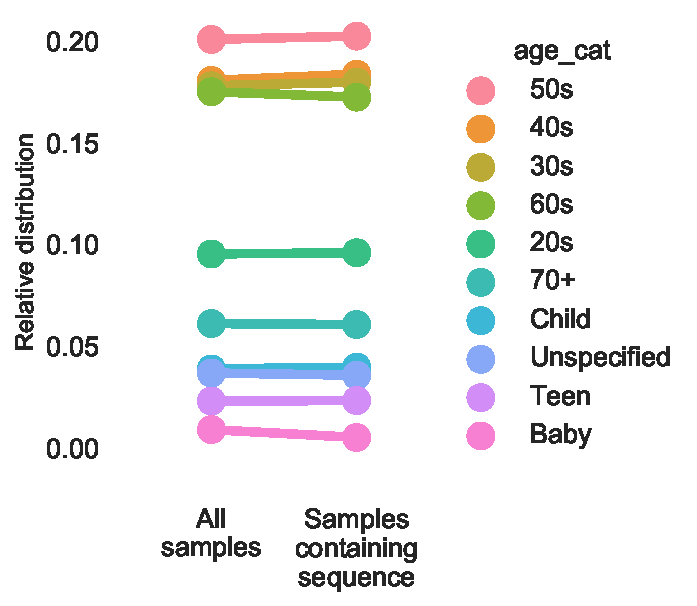
\includegraphics[height=4.5cm]{age_cat.pdf} & 
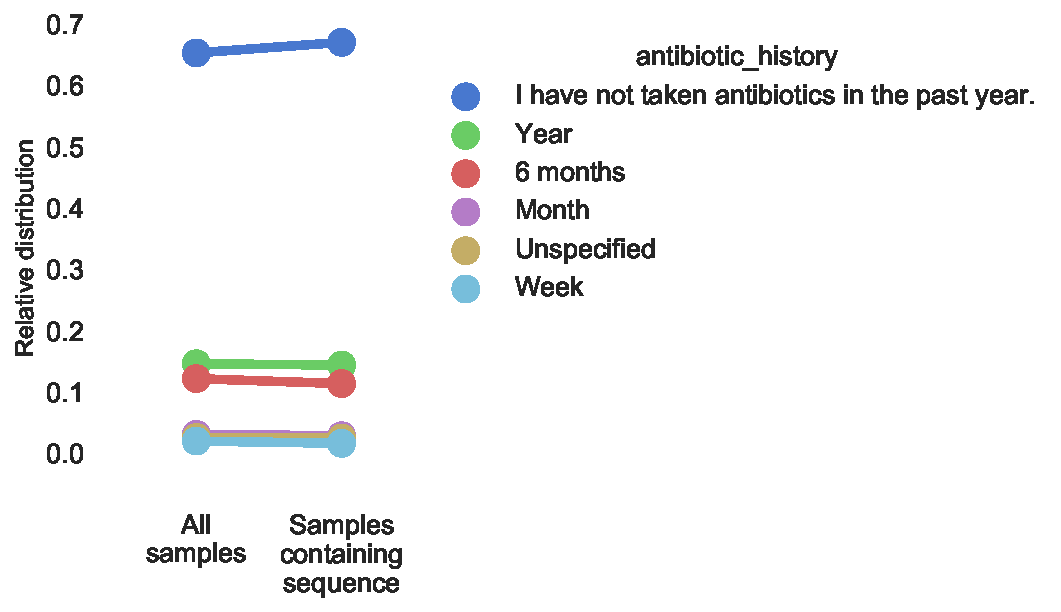
\includegraphics[height=4.5cm]{antibiotic_history.pdf}\\ 
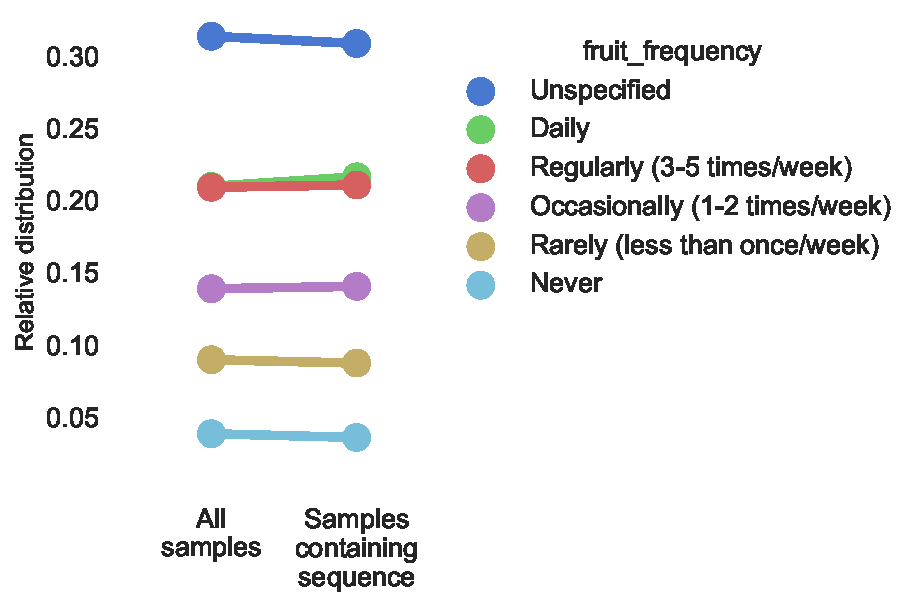
\includegraphics[height=4.5cm]{fruit_frequency.pdf} &
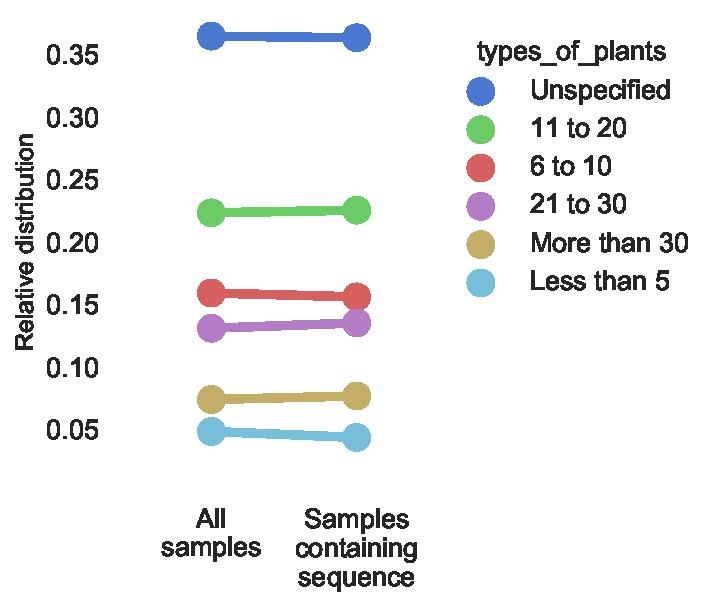
\includegraphics[height=4.5cm]{types_of_plants.pdf}
\end{tabular}

\end{raggedright}


\begin{center}
	\copyright{} 2017 American Gut Project
\end{center}

%\end{framed}


\end{document}  
